\documentclass{beamer}

\usepackage{amsmath, amssymb}
\usepackage{tikz-cd}
\usepackage{xcolor}
\usepackage{graphicx}

\title{MAT102 - College Algebra - Polynomial and Rational Functions}
\subtitle{3.1 Quadratic Functions and Applications \cite{miller2016college}}
\author{\textbf{Miraj Samarakkody}}
\institute{Tougaloo College}
\date{Updated - \today}

\begin{document}

\begin{frame}
    \titlepage
\end{frame}

\begin{frame}{Graph a Quadratic Function Written in Vertex Form}
    \begin{itemize}
        \item A function of the form \(f(x) =mx+c ~ (m \ne 0)\) is a linear function. \pause
        \item The function defined by \(f(x) = ax^2 +bx + c ~(a \ne 0) \) is called a \textbf{quadratic function.}  \pause
    \end{itemize}
    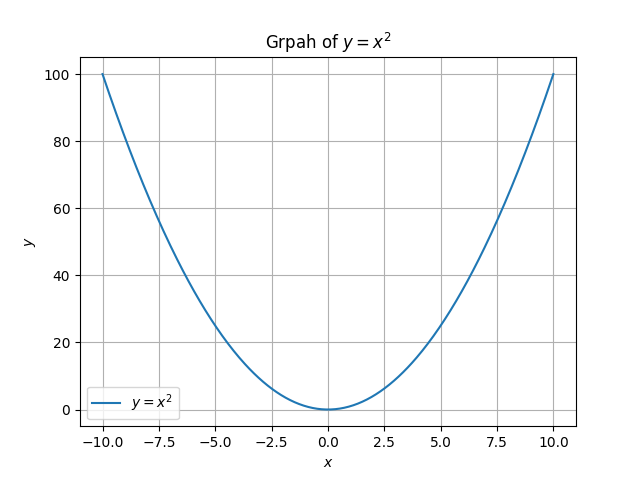
\includegraphics[scale=0.5]{figs/Figure_1.png}\pause
\end{frame}

\begin{frame}
    \frametitle{Graph a Quadratic Function Written is Vertex Form}
    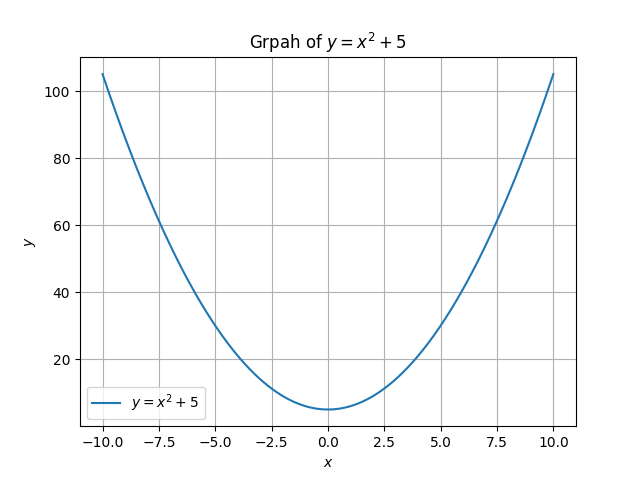
\includegraphics[scale=0.5]{figs/Figure_2.png}

    

\end{frame}

\begin{frame}
    \frametitle{Graph a Quadratic Function Written is Vertex Form}
    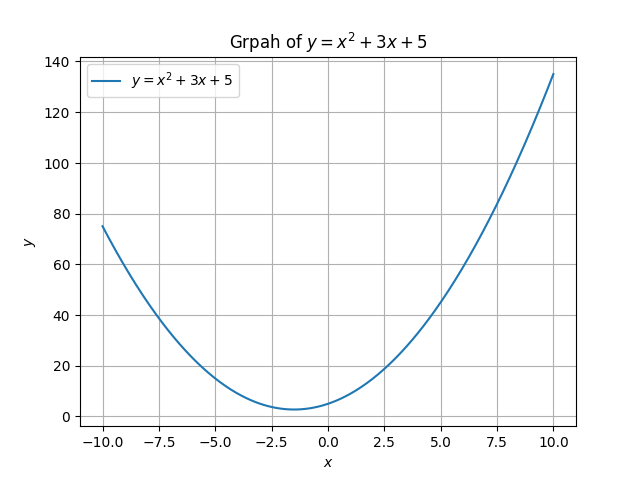
\includegraphics[scale=0.5]{figs/Figure_3.png}
\end{frame}

\begin{frame}
    \frametitle{Quadratic Function}

    A function defined by \(f(x) = ax^2 +bx +c~ (a \ne 0)\) is called a \textbf{quadratic function}. By completing the square, \(f(x)\) can be expressed in \textbf{vertex form} as \(f(x)= a(x-h)^2+k\).\pause
    \begin{itemize}
        \item The graph of \(f\) is a parabola with vertex \((h,k)\). \pause
        \item If \(a>0\), the parabola opens upward, and the vertex is the minimum point. The minimum value of \(f\) is \(k\). \pause
        \item If \(a<0\), the parabola opens downward, and the vertex is the minimum point. The minimum value of \(f\) is \(k\). \pause
        \item The axis of symmetry is \(x=h\). This is the vertical line that passes through the vertex. 
    \end{itemize}

\end{frame}

\begin{frame}{Example - Analyzing and Graphing a Quadratic Function}
Give \(f(x)=-2(x-1)^2+8\),
\begin{enumerate}
    \item Determine whether the graph of the parabola opens upward or downward. \pause
    \item Identify the vertex. \pause 
    \item Determine the \(x-\)intercepts. \pause 
    \item Determin the \(y-\)intercepts. \pause
    \item Sketch the function. \pause
    \item Determine the axis of symmetry. \pause  
    \item Determine the maximum or minimum value of \(f\).\pause
    \item Write down the domain and range in interval notaion. 
\end{enumerate} 

    
\end{frame}





\begin{frame}
    \frametitle{References}
    \bibliographystyle{plain} % or another style like unsrt, alpha, etc.
    \bibliography{reference}  % omit the .bib extension
\end{frame}

\end{document}

